\chapter{EightPuzzle with Java Beans}

\section{About folders content}

The assignment development was tracked using git. The repository is available at \href{https://github.com/frenzis01/AP-assignments}{github.com/frenzis01/AP-assignments}.\\
The folder of the first exercise is \texttt{assignment1/ex1}.
 
There are many subdirs which mirror the structure of the NetBeans project, but only the \texttt{.java} class files are actually present, for ease of reading.
There is also the \texttt{.jar} file (renamed to \texttt{.raj}) of the app which may be tested as it is.
% // TODO
There is also a \texttt{NetBeans.zip} archive resulting from the export of the NetBeans project, which contains the source code and the NetBeans project files; it may be imported in NetBeans to navigate and test project from the IDE.


\section{Main Design Choices}

Components are exactly the ones required by the assignment: \lstinline|EightTile|, \lstinline|EightBoard|, \lstinline|EightController| and \lstinline|Flip|, with the only addition of a simple wrapper class \lstinline|IntWrapper| under the \lstinline|utils| package.

\subsection{\texttt{position} and \texttt{label} attributes}
\begin{paracol}{2}
   \colfill
   It is important to keep in mind that \lstinline|EightTile| components are positioned as in Fig. \ref{fig:netBeans_board}.
   Every \lstinline|EightTile| is instantiated with the expected corresponding \lstinline|position|, i.e. \lstinline|eightTile6| $ \rightarrow $ \lstinline|eightTile6.position = 6|.

   \lstinline|EightTiles| \textit{never} ``move'' in the board and neither their \lstinline|final position| attribute ever changes, only the \lstinline|label| attribute is changed throughout the game, mimicking the sliding of the tiles.

   \note{\lstinline|label| is private, there is no getter and no setter. It is changed only when invoking \lstinline|labelRequest()| (which fires a vetoable change) and upon receival of \lstinline|"swapOK"| and \lstinline|"restart"| events.}
   \colfill
   
   
   \switchcolumn
   \begin{figure}[htbp]
      \centering
      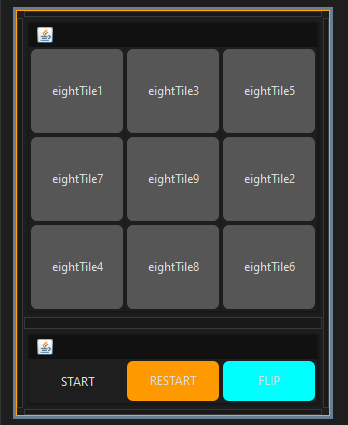
\includegraphics[width=0.4\columnwidth]{images/netBeans_board.png}
      \caption{\lstinline|EightTile| components organized in the \lstinline|EightBoard| grid}
      \label{fig:netBeans_board}
   \end{figure}
\end{paracol}

\subsection{Observer pattern}

The interaction between components is based on events and listeners, following the Observer pattern.\\
\lstinline|EightTile.label| is a \textit{Constrained Property} which fires a \lstinline|PropertyChangeEvent| by invoking \lstinline|fireVetoableChange(...)| on the \lstinline|EightController| instance, which is responsible for ensuring that only legal changes are allowed.
The three scenarios for a \lstinline|label| change are:
\begin{enumerate}
   \item \textit{Tile got clicked}: clicked \lstinline|EightTile| may move to the \textit{hole} (i.e. \lstinline|EightTile| whose \lstinline|label == 9|), if adjacent to it.
   \item \textit{Flip button got clicked}: tiles in position 1 and 2 are swapped, if the \textit{hole} is in the middle (\lstinline|position == 5|) 
   \item \textit{Restart button got clicked}: tiles receive a permutation and infer their new label (\lstinline|eightTiles[i].label := permutation[i]|); in this case, such change is not vetoed.
\end{enumerate} 

\subsection{Events}
\subsubsection{Clicking a Tile}
When an \lstinline|EightTile| gets clicked it attempts to swap its position to the hole. To do so, sets the property \lstinline|requestedLabel = 9| (i.e. hole), and executes \lstinline|EightTile.labelRequest(9)| which fires a \lstinline|PropertyChangeEvent| with \lstinline|propertyName = "label"|, \lstinline|oldValue = position| and \lstinline|newValue = 9|.

\framedt{Bending the rules}{
   Considering the signature Lst. \ref{fig:netBeans_board} below, we might say that the parameters are not exactly used as their name suggests, and we'd probably be right \smiley.\\
   In fact \lstinline|oldValue| is used to pass the \textit{position} of the tile, while the \lstinline|newValue| is used to pass the new \textit{label} of the tile.\\
   I chose to pass the position in the event to avoid making the Controller check the position of the requesting tile using methods (e.g. \lstinline|((EightTile) pce.getSource()).getPosition()|) as the assignment requires.
   \note{It is needed to wrap position because in case \lstinline|oldValue == newValue| the event is not fired, and it is not unlikely that \lstinline|position == newLabel|.}
   }
   {
      \begin{lstlisting}[label=lst:fireVetoableChange,captionpos=b,caption={How \lstinline|fireVetoableChange| is used in \lstinline|EightTile|}]
         // Signature of fireVetoableChange
         fireVetoableChange(String propertyName, Object oldValue, Object newValue)
         // How it is used in EightTile
         this.mVcs.fireVetoableChange(propertyName, new IntWrapper(this.position), newLabel);
      \end{lstlisting}
   }

\lstinline|EightController| which a \lstinline|vetoableChangeListener|, checks if the requesting tile is adjacent to the hole, and if so, it allows the change, otherwise throws an exception.
In case an \lstinline|EightTile| successfully moves, fires an \lstinline|ActionEvent("swapOK")|\footnote{Almost analogous behaviour may be obtained by using \lstinline|PropertyChangeEvent|}, which is listened by all other tiles, so that the tile ---typically the \textit{hole}, unless it's a \textit{Flip}--- which has been swapped can update its label.
The requested label is obtained by listener by invoking on the event source \lstinline|getClientProperty("requestedLabel")|.
\note{7 tiles out of 8 listen to the event uselessly, the clicked tile could send it only to the hole, but it would require for it to have a reference to the tile currently holding the hole; for simplicity and readability, I chose to make all tiles listen to the event.}

\subsubsection{Restarting a Game}
The restart button generates an array representing a permutation of the labels ---with the $i^{th}$ element being the label for the \lstinline|EightTile| in $i^{th}$ position--- and puts it in a property \lstinline|"permutation"|, and emits an event \lstinline|"restart"|, which is listened by both the tiles to update their label, and by the Flip button to update the position of the hole.

\note{The board is initialized by mimicking a click on the restart button.}

\section{Flip Button}

The \lstinline|Flip| button is not aware of the labels of the tiles, it only knows the position of the hole, and the labels of the tiles in position 1 and 2; the button listens for \lstinline|"restart"| and \lstinline|"swapOK"| events, to update its state.

When clicked, it emits an event \lstinline|"flip"|, which is listened by the \lstinline|EightController|, which checks if the hole is in the middle, if so the button updates its \textit{internal state} (\lstinline|label1| and \lstinline|label2|).\\
To implement the actual Flip on the tiles, the label update is delegated to the tiles theirselves by simply setting the \lstinline|"requestedLabel"| property of the tile in position 1 to the label of the tile in position 2, and then mimicking a click on the tile in position 1.

\begin{lstlisting}
   // Code taken from the flip1 actionListener in EightBoard
   if (flip1.flipTiles()){
      // label1 and label2 inside flip1 have been successfully swapped!
      eightTile1.putClientProperty("requestedLabel", flip1.getLabel1());
      eightTile1.doClick();
   }
\end{lstlisting}

The change will be again vetoed by \lstinline|EightController| which will notice that the requested label is not the hole, and will allow the change.
\note{The controller checks that the hole is in the middle even if at this point, the hole should be there; this double check is not necessary}